% F2 method diagram (minimal TikZ -> fig_method.pdf). Pure CM Roman to avoid BasicTeX font-gen loops.
\documentclass{article}
\usepackage[paperwidth=44cm,paperheight=20cm,margin=1cm]{geometry}
\usepackage{tikz}
\usetikzlibrary{positioning,arrows.meta}
\pagestyle{empty}
\begin{document}\noindent
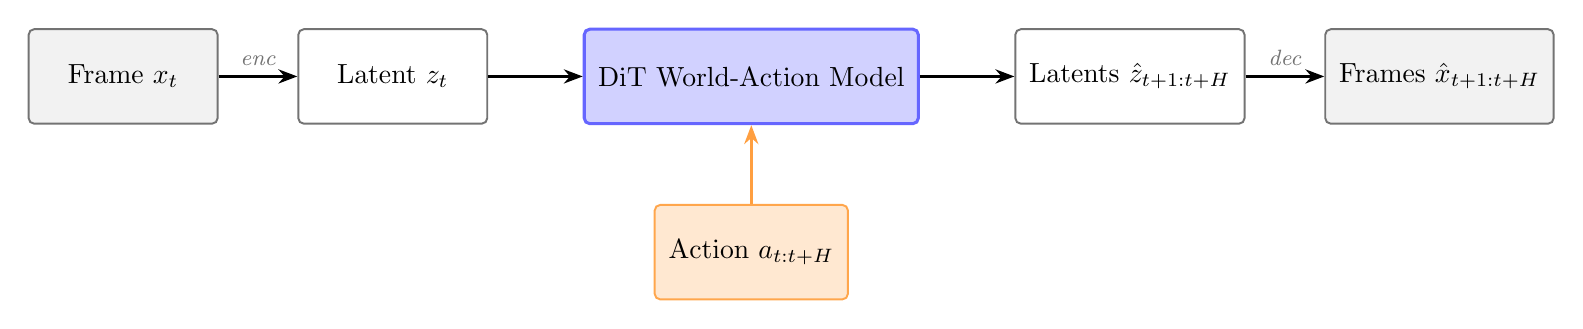
\begin{tikzpicture}[
  box/.style={rounded corners=2pt, draw=black!55, line width=0.7pt, align=center, inner sep=5pt,
              minimum height=12mm, minimum width=24mm, fill=white},
  frame/.style={box, fill=black!5},
  core/.style={box, fill=blue!18, draw=blue!60, line width=1.1pt, minimum width=36mm},
  act/.style={box, fill=orange!18, draw=orange!70},
  ar/.style={-{Stealth[length=2.4mm]}, line width=0.9pt},
  lbl/.style={font=\itshape\footnotesize, text=black!55}
]
\node[frame] (xt) {Frame $x_t$};
\node[box, right=10mm of xt] (zt) {Latent $z_t$};
\node[core, right=12mm of zt] (dit) {DiT World-Action Model};
\node[box, right=12mm of dit] (zf) {Latents $\hat z_{t+1:t+H}$};
\node[frame, right=10mm of zf] (xf) {Frames $\hat x_{t+1:t+H}$};
\draw[ar] (xt) -- node[lbl,above]{enc} (zt);
\draw[ar] (zt) -- (dit);
\draw[ar] (dit) -- (zf);
\draw[ar] (zf) -- node[lbl,above]{dec} (xf);
\node[act, below=10mm of dit] (act) {Action $a_{t:t+H}$};
\draw[ar,orange!75] (act) -- (dit);
\end{tikzpicture}
\end{document}
